\section{Introduction}
Entanglement-based quantum key distribution (QKD) relies on a steady source of photon pairs. The first step in establishing a key in such a scheme is the assignment of photodetection events to entangled photon pairs. Ho et al. (2009) \cite{ho2009clock} introduced an algorithm for coincidence matching under a constant time offset ($\Delta T$) and a constant frequency difference ($\Delta u$). However, for satellite-based photon pair sources, an element of Doppler shift causes the relative clock frequency between the satellite and groundstation to vary in time ($\Delta T(t),\Delta u(t)$). The complexity from Doppler shift rates at different angles of elevation can cause this cross correlation to be spread out over thousands of time bins. This note introduces two methods for correcting Doppler effects in satellite-to-ground coincidence matching. 

\subsection{Time stamping a satellite SPDC source}

We consider a setup where a spontaneous parametric down conversion (SPDC) source on a satellite is time-stamped by two individual time-stamp cards with a relative clock drift of 165$\mu$s/s (Fig \ref{fig:spdc_source}).

\begin{figure}[ht!]
	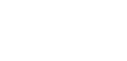
\includegraphics[width=\linewidth]{assets/spdc_source}
	\caption{Idlers and 1\% of signal photons are time-stamped on the satellite. The rest of the signal photons are transmitted to ground.}
	\label{fig:spdc_source}
\end{figure}

\newpage

\subsection{Propagation delay}
We introduce a propagation delay for each time-stamp based on pair generation time. When the elevation angle is at its maximum 90$^\circ$, we define that $t$ is 0 seconds. Assuming that the satellite is in a circular orbit at altitude $h = 500$km, with a carrier frequency of $f_c = 1$MHz, a simplified expression for the carrier propagation delay can be given by:

\begin{figure}[ht!]
	\begin{minipage}{.5\textwidth}
	\centering
	\includegraphics[width=0.75\linewidth]{assets/orbit.png}
	\label{fig:orbit}
	\end{minipage}%
	\begin{minipage}{.5\textwidth}
		\begin{align}
		V &= \sqrt{\frac{R^2}{r} \cdot g}, \label{eq1} \\
		\gamma &= \frac{V \cdot t}{r}, \label{eq2} \\
		\theta &= \arccos\Big(\frac{r\sin\gamma}{s}\Big), \label{eq3} \\
		s &= \sqrt{R^2 + r^2 - 2Rr\cos(\gamma)}, \label{eq4}\\
		f_d &= f_c \Big(\frac{V}{c} \cos\theta\Big). \label{eq5}
		\end{align}
	\end{minipage}
	\caption{A simplified schematic of the satellite's orbit.}
\end{figure}

\noindent where $R$ is the Earth's radius, $r = R + h$, $g$ is gravitational acceleration, and $c$ is the speed of light. Equation (\ref{eq1}) is the velocity of the satellite; (\ref{eq2}) is its orbital phase angle $\gamma$; (\ref{eq3}) is its angle of elevation $\theta$; (\ref{eq4}) is its distance from the ground station $s$; and (\ref{eq5}) is the Doppler shift of the carrier signal from the satellite.

Using this model, we specify an absolute time offset of 
\begin{equation}
\Delta t = \frac{s(t)}{c}, \label{eq6}
\end{equation}
where distance is calculated for each pair generation time in orbit (Fig \ref{fig:doppler_shift}(a)). 

\begin{figure}[ht!]
	\centering
	\begin{subfigure}[t]{0.49\linewidth}
		\centering
		\includegraphics[height=4cm]{assets/distance.png}
		\subcaption{}
	\end{subfigure}
	\begin{subfigure}[t]{0.49\textwidth}
		\centering
		\includegraphics[height=4cm]{assets/doppler_shift.png}
		\subcaption{}
	\end{subfigure}
\caption{(a) Distance to ground station, (b) Doppler shift of carrier signal.}
\label{fig:doppler_shift}
\end{figure}

\subsection{Doppler shift} 
The Earth station's clock can have an offset $t_s$ from true UTC and a drift of this offset $\frac{dt_s}{dt}$ with time. Since the satellite is moving at a different speed relative to the ground-station, the relative frequency difference between satellite and ground-station clocks is Doppler shifted (Fig \ref{fig:doppler_shift_rate}). This is a more significant source of error than the propagation delay $\Delta t$ (eq. \ref{eq6}), by almost one order of magnitude (Fig \ref{fig:correlation_smear}(a) and \ref{fig:correlation_smear}(b)). 

\begin{figure}[ht!]
	\centering
	\includegraphics[width=0.95\linewidth]{assets/correlation_smear.png}
	\caption{Effect of Doppler shift and Doppler shift rate on photoevent sets. Trace (a) represents the event set $\{t_i\}$ on side  A, trace (b) an event  set $\{t′_j\}$ on side B  with a time offset $\frac{s(t)}{c}$ , but  the  same reference clock frequency. Trace (c) illustrates a set $\{t'_j\}$ with an additional relative frequency difference $\delta$ between both reference clocks. Image adapted from \cite{ho2009clock}.}
	\label{fig:correlation_smear}
\end{figure}

Since the stream of time stamps $\{t_i\}$ and $\{t_j\}$ on each side has no intrinsic time structure, it is difficult to distinguish a signal event from a background event in the frequency-shifted $\{t'_j\}$ (Fig \ref{fig:correlation_smear}(c)). 

The change in the Doppler shift over time is highest at $90^\circ$ elevation angle and can reach up to nearly 400 ns/s$^2$ (Fig \ref{fig:doppler_shift_rate}). This causes a change in relative clock drift over time. This stretch is of the order of microseconds per second (23 $\mu$s/s for Doppler, 165 $\mu$s/s for clock drifts) and it causes the cross correlation to be spread out thousands of time bins, making it difficult to distinguish a significant peak in the cross correlation.

\begin{figure}[ht!]
	\begin{minipage}{.5\textwidth}
		\centering
		\includegraphics[width=\linewidth]{assets/doppler_shift_rate.png}
		\caption{The change in Doppler shift.}
		\label{fig:doppler_shift_rate}
	\end{minipage}%
	\begin{minipage}{.5\textwidth}
		To correct for this, we introduce a second order term to our time shift equation:
		\begin{equation}
		\Delta t = \frac{s(t)}{c} + \delta \cdot t,
		\end{equation}
		
		where the Doppler shift $\delta$ is defined by (cf. eq. \ref{eq5})
		
		\begin{equation}
		\delta = \frac{V}{c} \cos\theta.
		\end{equation}
	\end{minipage}
\end{figure}

The former subsections used a simplified model of the Earth's orbit to introduce Doppler shift concepts. Numerically accurate calculations can be done using data from the Python \texttt{pyephem} package. 

